% Theoretical background

\chapter{Theoretical background}
In this chapter, basic principles and theories in fluid dynamics related to the problem of vortex current inside the pipeline are reviewed. These include theoretical backgrounds of internal flow in a circular pipe, flow motion in a curved pipe and vortex flow, which can be found in Fluid Mechanic textbook, peer-review articles, and journals. After considering theoretical literature review the subject, we identify the gap of related theory on subjects of the experiment.

\section{Internal flow in circular pipe}

\subsection{Reynolds number}

Reynolds number is one of the key points to define fluid properties, predict flow patterns in different fluid situations. It is expressed as a ratio of inertial forces and viscous forces in the fluid. 
\begin{align}
Re & = \frac{Inertial forces}{Viscous forces} = \frac{V_avg D}{\nu} = \frac{\rho V_avg D}{\mu} 
\end{align}

$V_{avg}$ is the average flow velocity ($m/s$); $D$ is the diameter of pipe ($m$); $\nu$ or $\frac{\mu}{\rho}$ is the kinematic \gls{viscos} of fluid ($m^2/s$). The transition flow from laminar to turbulent depends on the degree of disturbance of flow by surface roughness, pipe vibrations and fluctuations in upstream flow (p.349) \cite{cengel:book}. For Newtonian fluids, Reynolds number is:

\begin{table}[b]
\centering
\begin{tabular}{r l}
$Re$ $\leq$ $2300$ & laminar flow \\
2300 $\leq$ $Re$ $\leq$ $4000$ & transitional flow \\
$Re$ $\geq$ $4000$ & turbulent flow
\end{tabular}
\end{table}

\subsection{Laminar flow}

Laminar flow in the pipe has $Re$ $\leq$ $2300$ which is smooth and highly ordered motion moving in a straight line parallel to the surface. The flow is fully developed without any disruption if the pipe is sufficiently long enough (p.353) \cite{cengel:book}. There are no cross-currents perpendicular to the direction of flow, nor eddies or swirls of fluids. Laminar flow is a flow establishment indicated by high momentum diffusion and low momentum convection. Laminar flow is described as a novel flow which usually occurs under highly controlled condition.

\subsection{Turbulent flow}

In our investigation, the flow is turbulent as well as most of the encountered situations. In daily life, it can be seen under a form of waves, storm clouds, fast flowing rivers, etc. Turbulent flow with $Re \geq 4000$ which is usually chaotic and has rapid fluctuations (p.361) \cite{cengel:book}. In turbulent flow, the swirling eddies transport mass, momentum, and energy to other regions of flow much more rapidly than molecular diffusion, greatly enhancing mass, momentum, and heat transfer. Therefore, it usually has higher friction values, heat transfer, and mass transfer coefficients. 
\begin{wrapfigure}{r}{0.5\textwidth}
  \begin{center}
    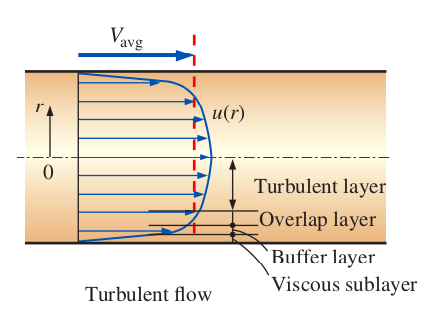
\includegraphics[width=0.48\textwidth]{turbulent}
  \end{center}
  \caption{Velocity profile of turbulent flow \cite{cengel:book}}
  \label{fig:turbu}
\end{wrapfigure}
Sometimes, there are unstable vortices in many sizes interacting with each other, which increase friction effects leading to drag effect. The drag effect makes the pump needed more energy to pump fluid through the pipe. This also resonates with the pipe or form \gls{cavit} that increase energy dissipation. While the velocity profile in laminar flow is parabolic, the velocity profile in turbulent flow develops fuller and has a sharp drop near pipe wall.  In the pipe, the thin layer next to the wall is called viscous sublayer (see figure \vref{fig:turbu}) where viscous effects are major. Next to it is the buffer layer where turbulent effects are getting significant but still affect largely by viscous layer. Above this layer is transition layer, in which the turbulent effects are getting stronger. 

\subsection{Major and Minor Losses}
In a typical piping system, the fluid goes through various components like fittings, valves, bends, elbows, reducer, etc, in addition to a straight section of piping. Major losses are defined by head loss or pressure loss in straight sections and minor losses occur in the other components of piping. 

\textbf{Pressure loss} is expressed as:
\begin{align}
\Delta P_L & = f \frac{L}{D} \frac{\rho V_{avg}^2 D }{2} 
\end{align}
$\frac{\rho V_{avg}^2 D }{2}$ is the dynamic pressure in the pipe; $f$ is the Darcy- Weisbach friction factor.  
The equivalent expression for pressure loss is well known as equivalent fluid column height or \textbf{head loss}. Head loss represents \textit{the additional height that the fluid needs to be raised by a pump in order to overcome the frictional losses in the pipe} (p.356) \cite{cengel:book}. It is obtained by:
\begin{align}
 h_L & =  \frac{\Delta P_L}{\rho g} = f \frac{L}{D} \frac{V_{avg}^2 }{2g}
\end{align}

In another hand, minor losses are usually asserted as loss coefficient $K_{\text{L}}$.  Loss coefficient depends on the geometry of component and the Reynolds number. However, Reynolds number is usually ignored. It is defined as:
\begin{align}
K_L & =  \frac{h_L}{\nu^2 / (2g)} 
\end{align}
In this case, $h_L$ is an additional irreversible head loss caused by insertion of the component.
When loss coefficient is available, \textbf{minor head loss} for the component can be also derived from $L_{equiv}$ as the equivalent length:
\begin{align}
 h_L & =  K_L \frac{V^2}{2g} = f \frac{L_{equiv}}{D} \frac{V^2 }{2g} \\
 L_{equiv} &= \frac{D}{f} K_L
\end{align}
The general total head loss in the piping system is determined from:
\begin{align}
 h_{L, total} & = h_{L, major} + h_{L, minor}
\end{align}

\section{Vortex Flow}
Vortex flow, a major component of turbulent flow, is a region of a fluid revolving around an axis line. The fluid flow velocity is strongest close to its axis and reduces in an inverse proportion to the distance of the axis. 
Vortex is best to describe by vorticity, a rotation vector of the fluid element defined by mathematically by a curl of velocity $\vec{V}$. 
\begin{wrapfigure}{r}{0.5\textwidth}
  \begin{center}
  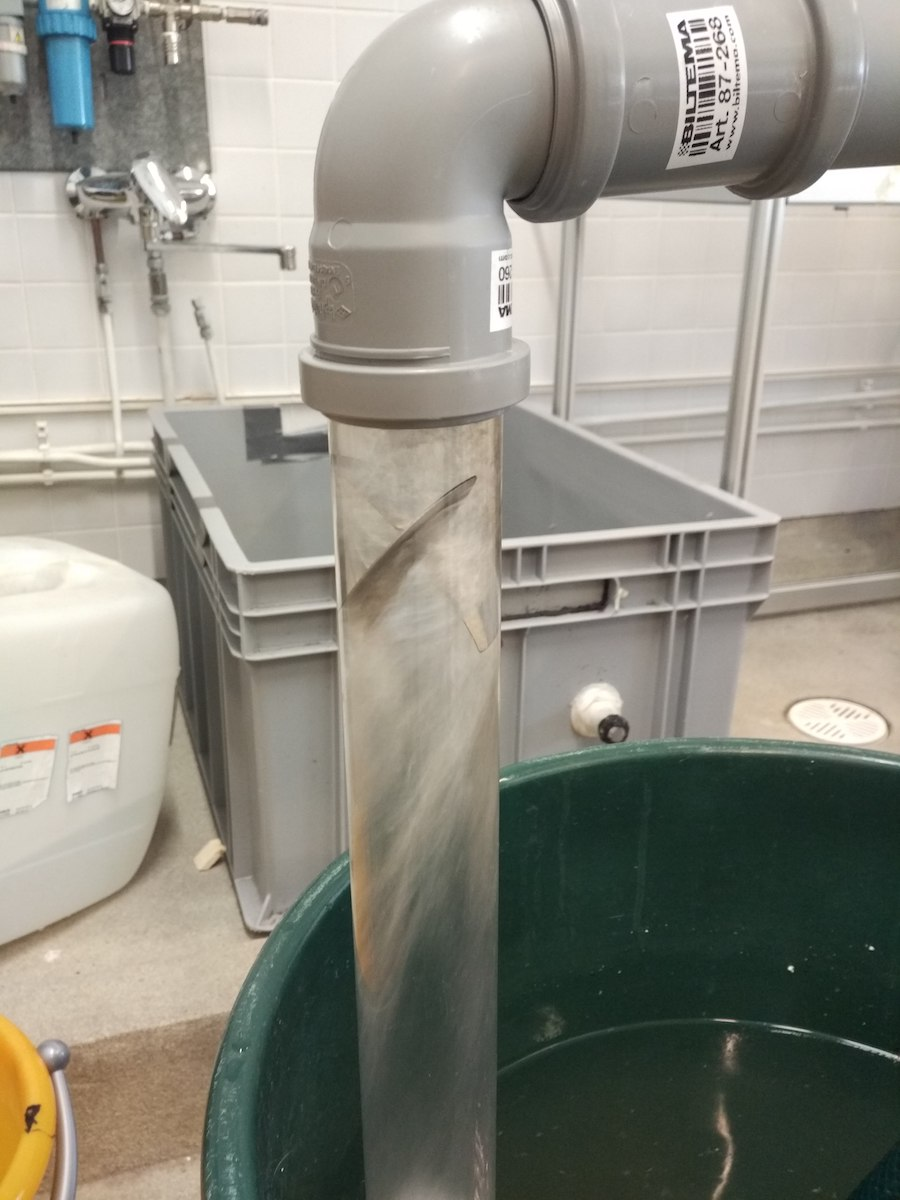
\includegraphics[width=6cm]{vortex}
   \end{center}
  \caption{Vortex current after Voxer wing with downward vertical direction}
  \label{fig:vortexf}
\end{wrapfigure}
There are two types of the vortex: irrotational vortex and rotational vortex. Rotational vortices happen when the vorticity at a point in the flow field is zero and the fluid particle occupying that point is rotating (p.156)\cite{cengel:book}. The fluid itself doesn't generate the vortex rotation but external or extra forces which apply on it to keep the motion going indefinitely. 
Irrotational vortices are also called free vortices. A vortex evolves fairly quickly toward the irrotational flow pattern, where the flow velocity is inversely proportional to the distance \cite{wiki:web}.
According to Bernoulli's principle (p.200) \cite{cengel:book}, the fluid motion in a vortex creates dynamic pressure. This dynamic pressure is lowest in its core region, around the axis, and develops when moving away from it. Figure \vref{fig:vortexf} presents the vortices after going downward through Voxer into a vessel in the test piping system. 


\section{Flow Motion in $90^{\circ}$ pipe bend}
From the knowledge in the section of minor loss, it is said that these losses would occur when going through the curved pipe. In real life condition, the flow motions through the curved pipeline are further than complicated being either laminar, transitional or turbulent and through the presence of swirling or pulsations \cite{curve:article}. When the fluid motion in straight pipe meets the curve, the fluid particle changes their main direction of motion. In the curved conduits, the centrifugal force ($U^{2} / R_{c}$, where U is the velocity and $R_{c}$ is the radius of curvature) induced from the bend will act stronger on the fluid close to the pipe axis than close to the walls. as the higher velocity fluid is next to the pipe axis. This is an adverse pressure gradient generated from the curvature with an increase in pressure, therefore a decrease in velocity close to the convex wall, and the contrary will occur towards the outer side of the pipe. 

\clearpage %force the next chapter to start on a new page. Keep that as the last line of your chapter!
